\documentclass{ximera}

\usepackage{accsupp} % For screen reader alt-text


% MATH -----------------------------------------------------------
\newcommand{\nats}{\mathbb N}
\newcommand{\ints}{\mathbb Z}
\newcommand{\rats}{\mathbb Q}
\newcommand{\reals}{\mathbb R}
\newcommand{\complex}{\mathbb C}
\newcommand{\powerset}{\mathscr P}

%-------------------------------------------------------------


\begin{document}

    \title{Introduction to Differential Equations}
    
    \maketitle

\begin{figure}[h]
    \centering
    \BeginAccSupp{ActualText={A direction field (aka a slope field)}}
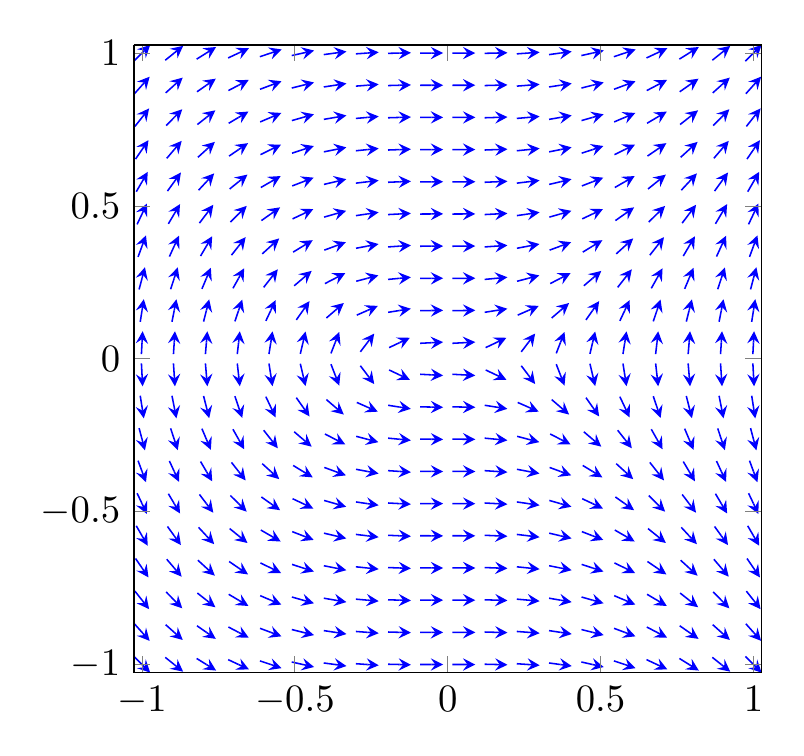
\begin{tikzpicture}[scale=1.4,
    declare function = {f(\x) = \x*\x/\y;} % Define which function we're using
    ]
    \begin{axis}[
        zmax = 1,
        zmin = 0,
        xtick = {-1,-0.5,...,1},
        axis equal image = true, % Unit vectors for both axes have the same length
        view = {0}{90}
        ]
        \addplot3[% Arrows' first-half
            blue,
            -stealth,
            domain  = -1:1,
            samples = 20,
            quiver  = {
                u=1/(2*sqrt(1^2 + f(x)^2)),
                v=f(x)/(2*sqrt(1^2 + f(x)^2)),
                scale arrows=0.075,
                },
        ] (x,y,0);
        \addplot3[% Arrow's second-half
            blue,
            domain  = -1:1,
            samples = 20,
            quiver  = {
                u=-1/(2*sqrt(1^2 + f(x)^2)),
                v=-f(x)/(2*sqrt(1^2 + f(x)^2)),
                scale arrows=0.075,
                },
        ] (x,y,0);
    \end{axis}
\end{tikzpicture}
    \EndAccSupp{}
    \caption{A direction field (aka a slope field)}
\end{figure}





\begin{large}

\vspace{1cm}

 An \underline{ordinary differential equation} (abbreviation $``$de")  is an equation involving derivatives of an unknown function  (usually $y$)  of one variable  (usually $x$ or $t$).

  A \underline{solution} to a de  is a function  that satisfies the de  on some open interval, 

 The graph of a solution is called a \underline{solution curve} of the de.    Any curve made of solution curves of a de is called an \underline{integral curve} of the de.  \\


  For example, $y=\sin{(t)}$ is a solution to the de $y''=-y$  on $(-\infty,\infty)$.\\

 For another example, $y=-\frac{1}{x}$ is a solution to $y'=y^2$  but only on open intervals not containing $x=0$.\\

 The \underline{order} of a de is the order of the highest-order derivative involved.  \\

 For example, the order of $y''=\frac{t^2}{y'}$ is $2$.\\


 Any first order equation can be solved for $y'=f(x,y)$ (or \\$y'=f(t,y)$).  

 If $f$ is defined on a region $R$ in the $xy$-plane then the \underline{direction field} (aka \underline{slope field}) for the de $y'=f(x,y)$ on $R$ is a graph consisting of short line segments (or arrows) with slope determined by $f(x,y)$ at each $(x,y)$ in $R$.\\

 % Having technology draw (approximate) slope fields is a powerful way to geometrically visualize a first order de. % At the top is the (approximate) slope field of $\displaystyle y'=x^2/y$ on $[-1,1]\times[-1,1]$.

\end{large}






\end{document}